\chapter{Covid}\label{chapter:Covid}
\addcontentsline{toc}{chapter}{Covid}

\section{Covid-19}\label{sec:covid19}
I coronavirus sono stati scoperti negli anni 60 e da allora i coronavirus sugli umani sono stati identificati a partire dal SARS-CoV nel 2002. La pandemia da Covid-19 
è causata da un nuovo ceppo virale chiamato SARS-CoV-2, un virus a singola elica di RNA della famiglia \emph{coronaviridae} (Fig. \ref{fig:coronavirus-struttura}). Dei 4 generi di coronavirus ($\alpha, \beta, \gamma, \delta$) fa parte dei $\beta-CoV$. 

\begin{figure}
	\centering
	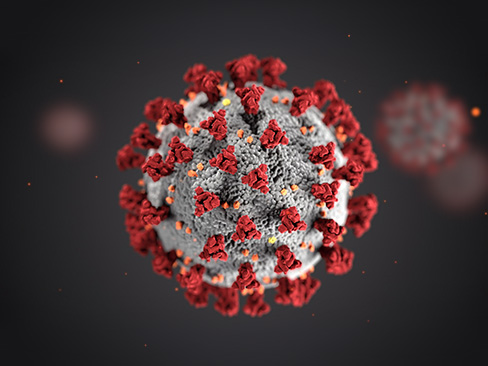
\includegraphics[width=0.4\textwidth]{Immagini/coronavirus.png}
	\caption{Struttura di un Coronavirus}
	\label{fig:coronavirus-struttura}
\end{figure}

Il genoma del virus, come citato in \cite{ijms22147425}, contiene quattro strutture proteiche: la proteina spike; la membrana; l'envelope; la nucleocapside; e da 16 proteine non strutturali (Nsp1-16). La proteina nucleocapside avvolge il genoma del RNA, incapsulato all'interno di un involucro associato alle proteine spike, envelope e membrana. 
La proteina spike media l'attaccamento del virus ai recettori dell'ospite, ma la approfondiremo nella prossima sezione. La membrana è la proteina più abbondante e definisce la forma dell'involucro virale. La proteina spike media l'interazione con i recettori della cellula ospite, che approfondiremo nella prossima sezione. La proteina membrana che è la più abbondante e definisce la forma dell'involucro virale. La proteina envelope si attiva durante il ciclo di replicazione e viene rilasciata nella cellula infetta in grandi quantità, ma solo una piccola parte viene incorporata all'interno del involucro virale. 

La replicazione del virus comincia con l'interazione della glicoproteina Spike con ACE2, il target espresso nelle cellule umane. 
Una volta che si viene a creare il legame, il virus entra nel citosol della cellula ospite. Dopodiché avviene la traduzione del gene per la replicazione dal RNA genomico e quindi poi la traduzione e l'assemblaggio dei processi di replicazione virale. Una volta conclusa questa fase avviene l'incapsulamento che porta alla formazione del virus maturo. Una volta completato il processo di assemblaggio viene trasportato sulla superficie cellulare e rilasciato per esocitosi.

Prima dell'epidemia del SARS-CoV erano già stati indivuduati due tipologie di coronavirus nell'uomo che però erano visti come le cause del raffreddore. Con la comparsa
nel 2012 di MERS-CoV e l'attuale SARS-CoV-2 è necessario studiare e comprendere appieno quelle che sono le proprietà e le caratteristiche di questo virus. 

\subsection{Storia}\label{subsec:storiacovid}
Come riportato da \cite{StoriaCovid} e da \cite{ReportCovid}, si è scoperta l'esistenza di questo virus il 31 Dicembre del 2019 quando l'OMS (Organizzazione Mondiale della Sanità) è stata informata di casi di polmonite di eziologia sconosciuta nella città di Wuhan provincia di Hubei Cina. Il nuovo corona virus è stato ufficialmente annunciato il 7 gennaio del 2020 e tre giorni dopo è stata resa pubblica la sequenza genomica. Sono state poi rilasciate altre sequenze genomiche, le quali tutte suggerivano la presenza di un virus strettamente legato al SARS-CoV. 

L'11 Febbraio del 2020 l'OMS ha definito la nuova polmonite indotta da coronavirus come malattia da corona virus 2019. Allo stesso tempo la Commissione internazionale di classificazione dei virus ha annunciato che il virus nominato provvisoriamente come 2019-nCoV veniva nominato come grave sindrome respiratoria acuta SARS-CoV2. Dopo che il patogeno è stato valutato sulla base della filogenesi, della tassonomia e della pratica consolidata, è stato definito un forte legame con il precedente SARS-CoV. 

L'inizio della pandemia è avvenuto quindi a Wuhan in Cina. In Italia si è sviluppato un focolaio autoctono che poi si è diffuso progressivamente in tutto il paese e in particolare nelle regioni del nord. Successivamente il virus si espanse in Europa e nel resto del mondo. L'OMS dichiarò l'inizio della pandemia l'11 Marzo del 2020, è poi storia di ogni giorno della pandemia che ha raggiunto milioni di persone. Si ritiene che comunque il tasso di mortalità del virus sia di circa il 3.5\%. 

\section{Glicoproteina Spike}\label{sec:glicoproteina}
La glicoproteina spike svolge un ruolo essenziale nell'attaccamento, nella fusione e nell'ingresso del virus nella cellula ospite. Una caratteristica dei coronavirus è quella di accedere alle cellule ospiti e poi dare inizio all'infezione attraverso la fusione delle membrane virali alle cellule. Come descritto in \cite{GlicoproteinaSpike}, la fusione della membrana viene mediata dalla membrana della glicoproteina spike e dal recettore affine della cellula ospite. Essendo in una posizione superficiale nella struttura del virus, ciò la rende un bersaglio diretto per le risposte immunitarie dell'ospite rendendola anche il principale bersaglio degli anticorpi. Data la sua importanza nella replicazione e fusione virale è al centro della maggior parte delle strategie vaccinali e degli interventi terapeutici. 

La glicoproteina Spike viene sintetizzata come precursore di una poliproteina sul reticolo endoplasmatico ruvido (RER). Il precursore non processato ospita una sequenza segnale del reticolo endoplasmatico (ER) situato nel terminale N, che indirizza la glicoproteina alla membrana RER. Durante la sintesi vengono aggiunte catene laterali di oligosaccaridi ad alto contenuto di mannosio. Poco dopo la sintesi i monomeri della glicoproteina trimerizzano, il che può facilitare il trasporto dall'ER al complesso di Golgi. Il complesso di Golgi è un organulo di composizione lipo-proteica con una delicata struttura nella cellula in posizione paranucleare che si occupa di rielabolare, selezionare ed esportare i prodotti del reticolo endoplasmatico. All'interno del complesso di Golgi la glicoproteina spike viene scissa proteoliticamente dalla furina cellulare o da proteasi simili in S1 e S2. La subunità di superficie S1, che attacca il virus al recettore della superficie della cellula ospite e la subunità S2 che media la fusione delle membrane cellulari alla cellula ospite. Anche dopo la fase di scissione le subunità S1 e S2 rimangono associate attraverso interazioni non covalenti in uno stato di profusione metastabile. La scissione è però necessaria per l'infettività virale ed è anche necessaria per un efficacie infezione delle cellule polmonari. Un segnale di recupero dell'ER costituito da un motivo conservato KxHxx assicura che la proteina matura si accumuli vicino al compartimento intermedio di Golgi dove guidata dall'interazione con la proteina di membrana (M) partecipano all'assemblaggio delle particelle virali. Una frazione delle proteine mature viaggia attraverso via secretoria fino alla membrana plasmatica, dove può mediare la fusione di cellule infette con cellule non infette per formare cellule giganti multinucleate.

\subsection{Struttura della proteina e funzione}\label{subsec:strutturaspike}
Come accenato nei precedenti paragrafi la glicoproteina spike svolge un ruolo fondamentale nell'infezione virale e nella patogenesi. Come descritto in \cite{LAHA2020104445}, la glicoproteina spike è una proteina omo-trimerica con due subunità S1 e S2. La subunità S1 è responsabile del legame ospite-recettore, mentre la subunità S2 aiuta nelle fusione delle membrane del virus e dell'ospite (Fig. \ref{fig:subunità}A). La proteina spike è divisa nelle due subunità, ma rimangono comunque legate tra di loro in modo non covalente nello stato di pre-fusione. É possibile dividere ulteriormente la subunità S1 in due sottodomini, ovvero il dominio N-terminale e in tre dominii C-terminale (Fig. \ref{fig:subunità}A).  

\begin{figure}
	\centering
	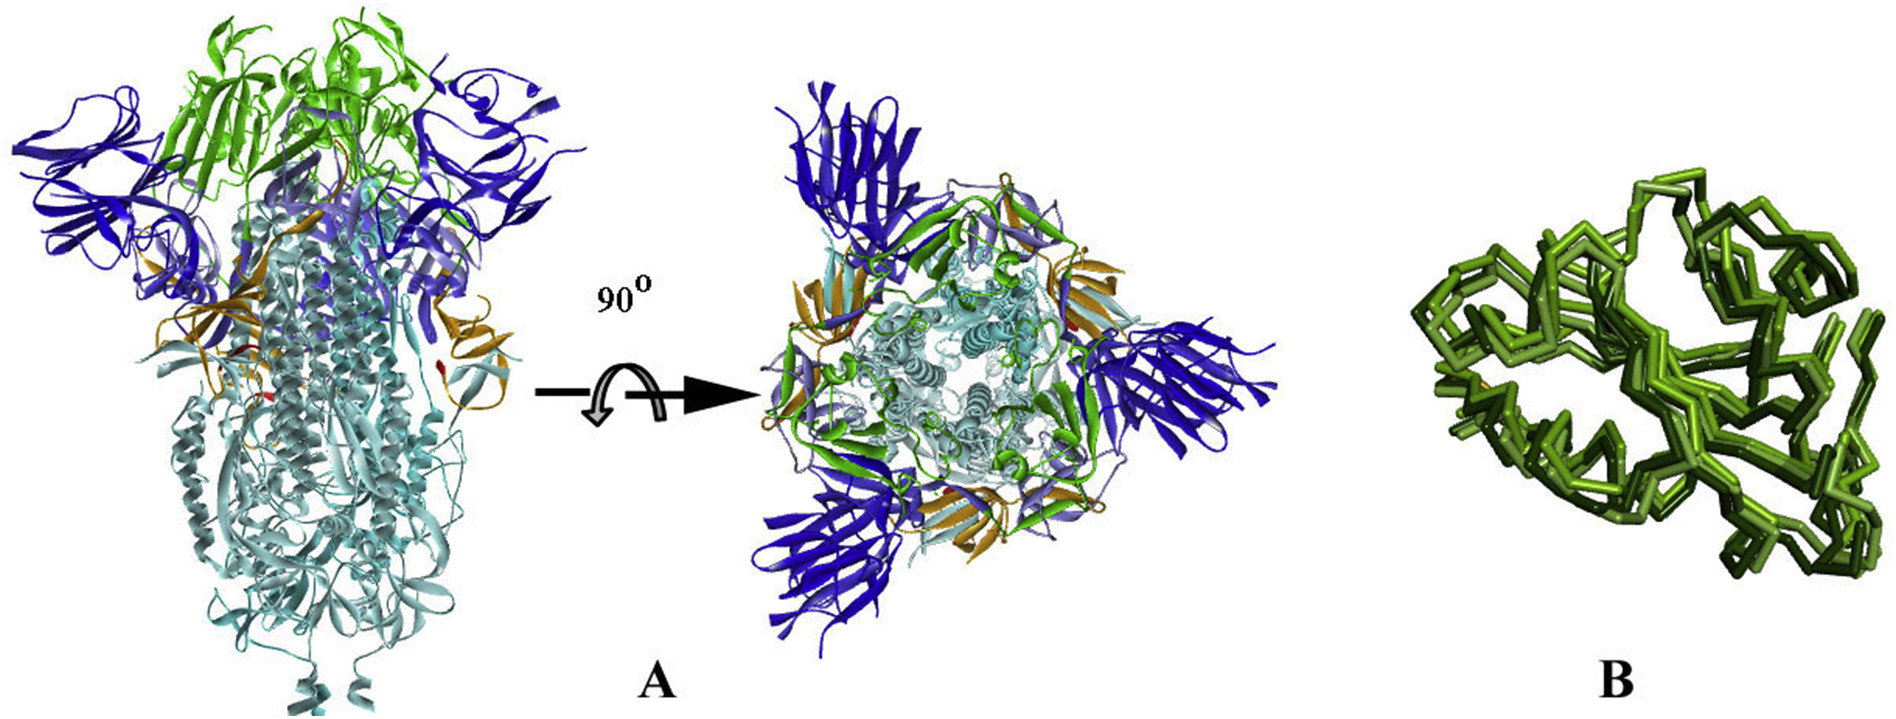
\includegraphics[width=0.9\textwidth]{Immagini/Subunita.png}
	\caption{Proteina spike: A, in due viste: NTD blu, RBD verde, CTD2 azzurro, CTD3 arancione, S1/S2 link rosso e S2 celeste. B, sovrapposizione degli RBD in conformazione chiusa e aperta; vi è anche lo stato di pre-fusione in colore verde sbiadito.}
	\label{fig:subunità}
\end{figure} 

Il CDT1, (Dominio C-terminale 1), è la regione principale della proteina spike per l'interazione ospite-recettore, ed è quindi definita Receptor Binding Domain (RBD). L'RBD subisce dei cambiamenti conformazionali durante il legame con il recettore umano che porta S1 in una configurazione aperta favorevole all'interazione. Confrontando poi le due conformazioni, quella inerte chiusa e quella attiva aperta, si scopre che l'RBD si muove come un corpo rigido attorno alla sua regione di collegamento con NTD e CTD2 (Fig. \ref{fig:subunità}B). Un simile cambiamento è visto anche nello stato di pre-fusione. 

Ci sono mutazioni senza senso nella proteina spike che vengono classificate come stabilizzanti e destabilizzanti in base ai cambiamenti di energia libera.

Come una tipica proteina di fusione di classe I la glicoproteina spike condivide caratteristiche strutturali topologiche e meccaniche comuni con altre proteina di fusione di classe I come la glicoproteina dell'involucro dell'HIV e l'emoagglutinina del virus dell'influenza. Essa è una macchina coformazionale che media l'ingresso virale riorganizzando da uno stato non unliganded metastabile, attraverso uno stato intermedio ad uno stato post fusione stabile. Da quando è stata resa pubblica la struttura sono state scoperte numerose strutture per i frammenti di trimero della glicoproteina spike negli stati pre e post fusione. 

\begin{figure}
	\centering
	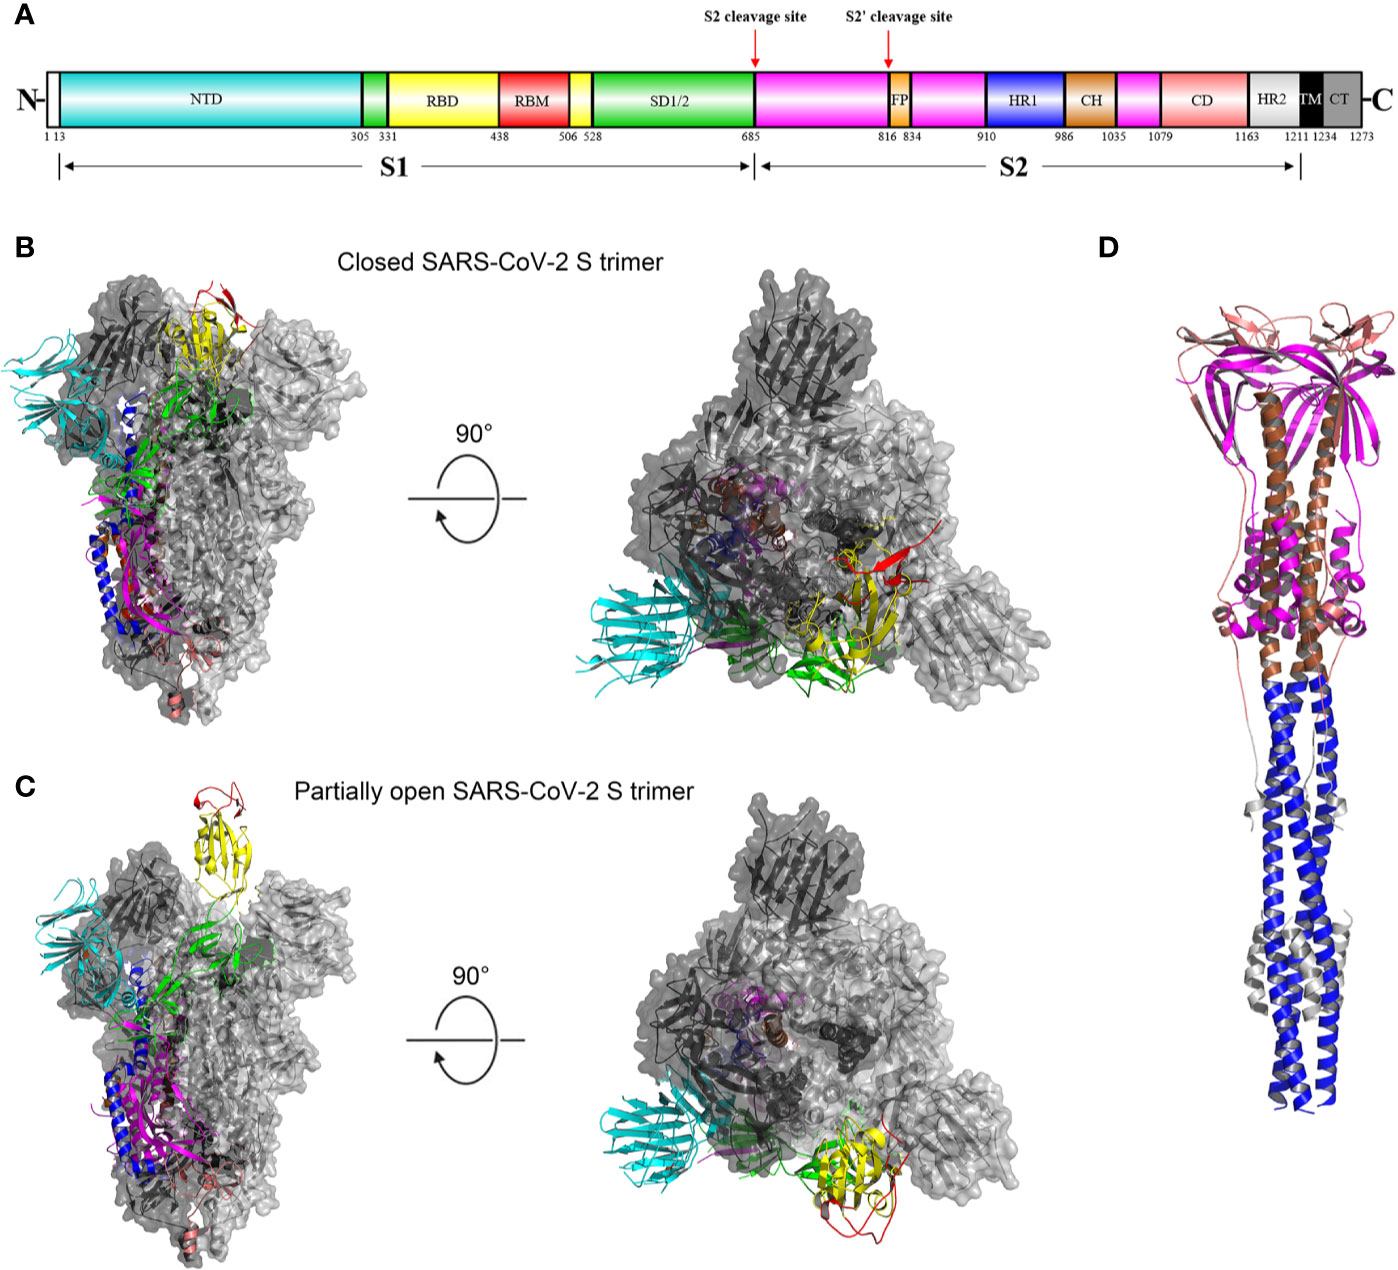
\includegraphics[width=0.7\textwidth]{Immagini/Composizione_strutturale.png}
	\caption{Struttura della glicoproteina spike}
	\label{fig:StrutturaMassima}
\end{figure}

La differenza strutturale tra queste due conformazioni risiede solo nella posizione di uno dei tre RDB. Quando tutti e tre gli RBD sono nella posizione giù il trimero risultante di ectodominio S assume una configurazione chiusa, in cui la superficie di legame del recettore dell'RBD S1 è sepolta tra i protomeri e non può essere accessibile dal suo recettore (Fig. \ref{fig:StrutturaMassima}B). Il trimero di ectodominio S con un singolo RBD nella posizione "up" assume una conformazione parzialmente aperta e rappresenta lo stato funzionale poiché la superficie di legame del recettore del RBD "up" può essere completamente esposta (Fig. \ref{fig:StrutturaMassima}C). La subunità S1 riposa mentre il trimero S2 stabilizzano quest'ultimo nella conformazione di pre fusione. Quando il trimero di ectodomionio adotta una conformazione parzialmente aperta l'RBD nella posizione "su" abolirà i contatti con la subunità S2 di un protomero adiacente, destabilizzando la conformazione parzialmente aperta. Ciò sarà vantaggioso per la dissociazione e faciliterà i riagganciamenti subiti per mediare l'ingresso virale. 

In particolare è noto che la pre fusione trimerica risiede principalmente in una configurazione chiusa che è conformazionalmente mascherata per eludere le neutralizzazioni mediate dagli anticorpi. Si può quindi pensare che le glicoproteine spike del covid-19 native su virioni maturi e infettivi che condividano una simile caratteristica di mascheramento conformazionale, nascondendo la superficie di legame del recettore.

\subsection{Scudo di glicani della glicoproteina spike}\label{subsec:scudospike}
Come nominato in precedenza la proteina spike del SARS-CoV-2 è fortemente circondata da glicani N-legati che sporgono dalla superficie del trimero. Sono stati visionati fino a 22 glicani N-legati che probabilmente svolgono un ruolo importante nel ripiegamento delle proteine e nell'invasione immunitaria dell'ospite come scudo glicano. Dei 22 potenziali disponibili per la glicosilazione, 14 vengono identificati come prevalentemente occupati da glicani di tipo complesso. I restanti invece risultano dominati da glicani di tipo oligomannosio che sono diversi da quelli fondati sulle glicoproteine dell'ospite. Per glicosilazione si intende una modifica della struttura della proteina da parte del complesso di Goigi, durante o in seguito ad un processo di sintesi proteica. Essa avviene per più motivi, uno dei quali è il raggiungimento del ripiegamento corretto, la può proteggere dall'attaccco di proteasi e aumenta la solubilità della molecola che viene dunque stabilizzata in tutti gli aspetti. Si può anche affermare che l'affinità di legame tra la proteina spike del SARS-CoV-2 e ACE2 non dipendono dalla glicosalinzione della stessa.

Nel caso di SARS-CoV-2, più recentemente è stato dimostrato che un potente anticorpo neutralizzante sia contro SARS-CoV che SARS-CoV-2, S309, riconosce un epitopo RBD contenente glicano altamente conservato. Queste osservazioni suggeriscono che le frazioni di carboidrati potrebberò essere immunogeniche ed evidenziano la necessità per gli immunogeni di mostrare i glicani importanti per il riconoscimento degli anticorpi neutralizzanti. Di conseguenza anche in questo caso è diventa fondamentale la ricerca in questo campo per i vaccini.


\section{RBD}\label{sec:rbd}
Come descritto in \cite{RBDSpike}, l'enzima di conversione dell'angiotesina 2 (ACE2) è un recettore di ingresso per SARS-CoV-2. Interazioni dettagliate tra il SARS-CoV-2 RBD e il suo recettore sono state rivelate da diverse strutture con ACE2. Come detto nella sezione precedente le subunità S1 e S2 sono responsabili del legame del recettore e della fusione della membrana. La subunità S1 è costituita da un dominio N-terminale e un dominio di legame o RBD. Nello stato di pre fusione, la proteina S esiste come omotrimero e subisce grandi cambiamenti conformazionali per controllare l'esposizione e l'accessibilità del RBD. Tutto questo avviene mediante un meccanismo di "su" e "giù", la differenza sta nel rendere accessibile o inaccessibile il recettore. La struttura del nucleo RBD quando è lagata ad ACE2 è costituita da un foglio $\beta$ antiparallelo a cinque filamenti intrecciati con eliche e anelli di collegamento corti.

\begin{table}[H]
	\centering
	\fontfamily{ptm}\selectfont
	\begin{tabularx}{0.85\textwidth}{|l|l|l|l|l|l|l|l|}
		\hline
		\textbf{\small hACE2} & \small Q24 & \small D30 & \small E35 & \small E37 & \small D38 & \small Y41 & \small Q42 \\ \hline
		\textbf{\small SARS-CoV-2} & \small N487 & \small K417* & \small Q493 & \small Y505 & \small Y449 & \parbox{0.6cm}{\small T500/\\N501} & \parbox{0.65cm}{\small G446/\\Y449 }\\ \hline
		& & & & & & & \\ \hline
		\textbf{\small hACE2} & \small Y83 & \small Q325 & \small E329 & \small N330 & \small K353 & \small R393 &\\ \hline
		\textbf{\small SARS-CoV-2} & \parbox{0.6cm}{\small Y489/\\N487} &  &  &  & \small G502 & \small Y505 &  \\ \hline
	\end{tabularx}
	\normalfont
	\caption{Tabella che riassume i principali residui che formano legami idrogeno e ponti salini tra ACE2 e SARS-CoV-2.}
	\label{tab:rtablega}
	\smallskip
	\begin{tablenotes}
		\item[\dag] Il residuo che forma ponti salini è contrassegnato con un asterisco.		
	\end{tablenotes}
\end{table}

\begin{figure}
	\centering
	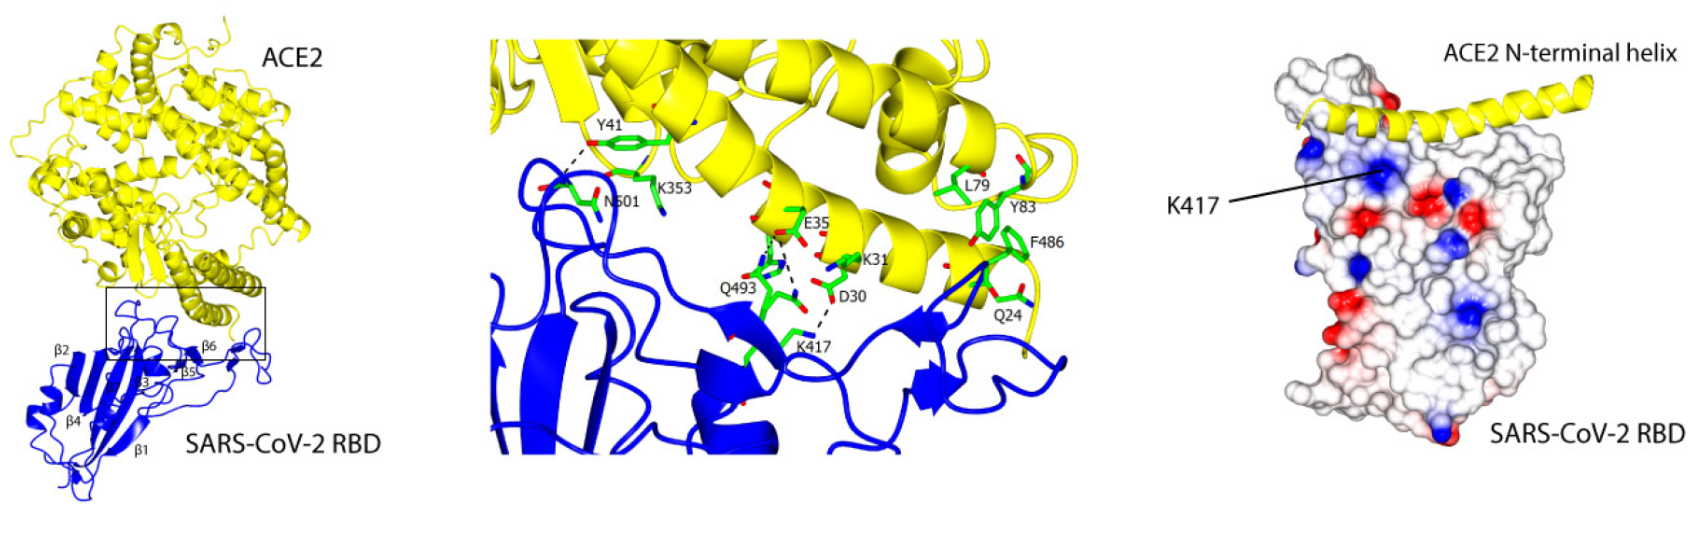
\includegraphics[width=0.7\textwidth]{Immagini/RBD-ACE2.png}
	\caption{SARS-CoV-2 RBD/ACE2. L'immagine a sinistra mostra la struttura complessiva del SARS-CoV-2(blu) legata a ACE2(giallo). L'immagine centrale mostra in dettaglio alcuni legame idrogeno e un ponte salino tra SARS-CoV-2 e ACE2. Nell'immagine sulla destra viene mostrata la mappa del potenziale elettrostatico del SARS-CoV-2 RBD con l'elica N-terminale di ACE2. Il dettaglio lo si può trovare nella Tab. \ref{tab:rtablega}}
	\label{fig:RBDstructure}
\end{figure}

Questa struttura centrale del foglio $\beta$ è ulteriormente stabilizzata da 4 legami di di solfuro. Tra i filamenti centrali c'è una regione estesa contenente 2 filamenti $\beta$ corti, le eliche e gli anelli. Questa regione è il motivo legante il recettore (RBM) che contiene la maggior parte dei residui responsabili dell'interazione con ACE2. Quando complessato con ACE2, l'RBM si ripiega in una superficie concava che ospita l'$\alpha$-elica N-terinale di ACE2. E' proprio in questa superficie che diversi residui di RBM stabiliscono interazioni specifiche e non specifiche con i residui di ACE2. Dai dati disponibili riguardo alla struttura sembrerebbe che la struttura centrale sia abbastanza stabile, mentre l'RBM risulta molto dinamico e non definito strutturalmente, a meno che non sia legato ad altre proteine come ACE2. Come citato in \cite{ijms22147425}, c'è un'elevata somiglianza tra l'RBD del SARS-CoV e l'RBD del SARS-CoV-2. Comparando gli RBD di SARS-CoV-2 e SARS-CoV, si nota che un numero maggiore di residui dell'RBD di SARS-CoV-2 interagiscono con ACE2, il che potrebbe spiegare la sua affinità di legame 10 volte superiore. Come si può notare in Fig. \ref{fig:RBDstructure},
K417 si trova al di fuori dell'RBM e forma una connessione a ponte salino con D30 di ACE2. K417 si può vedere come un cerotto carico positivamente sulla superficie di RBD che si collega all'Asp caricato negativamente di ACE2, per ottenere un legame più forte.

Durante il corso della pandemia sono state segnalate un numero significativo di mutazioni naturali della proteina Spike. Molte delle mutazioni sono state identificate nel RBD, alcune delle quali hanno dato origine a varianti virali. Si ritiene che molte di queste mutazioni RBD aumentino l'affinità di legame per ACE2 o riescono ad ingannare in modo migliore gli anticorpi monoclonali.  

I vaccini che sono stati elaborati nel corso della pandemia vanno proprio ad agire in questa zona tra RBD e ACE2, cercando di impedire che avvenga il contatto e che quindi impedire di conseguenza l'ingresso del virus all'interno dell'ospite.
